% Homework template for Algorithm Analysis and Design
% UPDATE: September 20, 2019 by Xu Rongchen
\documentclass[a4paper]{article}
\usepackage{ctex}
\ctexset{
proofname = \heiti{证明} %% set proof name
}
\usepackage{amsmath, amssymb, amsthm}
% amsmath: equation*, amssymb: mathbb, amsthm: proof
\usepackage{moreenum}
\usepackage{mathtools}
\usepackage{url}
\usepackage{bm}
\usepackage{enumitem}
\usepackage{graphicx}
\usepackage{subcaption}
\usepackage{booktabs} % toprule
\usepackage[mathcal]{eucal}

\usepackage[thehwcnt = 1]{iidef} % set homework count
\usepackage{longtable}


\thecoursename{高等计算机网路}
\theterm{2020年秋季学期}
\hwname{论文阅读}
\slname{\heiti{解}}
\begin{document}
\courseheader
\theusername{徐荣琛}
\thestuno{2019214518}
\theinstitute{软件学院}

\info


  
  % \setlength{\itemsep}{3\parskip}
  %% Homework Start here:
  %% \item to enumerate the problem ID: Format as 'HomeworkID.ProblemID'
  %% \begin{solution} XXXX \end{solution} is to make a solution
  %% \begin{proof} XXXX \end{proof} is to make a proof
  %% Suggest to use \input{path} command
\vspace{-15pt}
\begin{center}
  \begin{tabular}{c|c} \toprule
    \textbf{专题} &路由协议安全 \\\midrule
    \textbf{题目} &On the Feasibility of Rerouting-based DDoS Defenses\\
    \textbf{作者} &Tran M, Kang M S, Hsiao H C, et al. \\
    \textbf{会议} &2019 IEEE Symposium on Security and Privacy \\\bottomrule
  \end{tabular}
\end{center}
  
\vspace{20pt}
\setlength{\parindent}{2em}

本篇论文的主要工作是论证了路由阻塞绕行技术(Routing Around Congestion,简称RAC)在
实际边界网关协议(BGP)中防御DDoS攻击的不可行性。

RAC防御DDoS攻击的核心是目的自治系统利用BGP路由毒化机制,向关键流量源提供一条新的、不受
洪泛攻击影响的路由旁路。例如在图\ref{fig:Denfense}中,目的自治系统D为了排除攻击受影响
W相关路由通路,并向关键流量源C提供新的路由旁路CXYZD,于是向临近的自治系统Z发布包含毒化W
的路由更新指令,随后网络逐步更新并收敛,C到D的路由通路即从原来的CXWZD迁移到了CXYZD。

\begin{figure}[h]\centering
  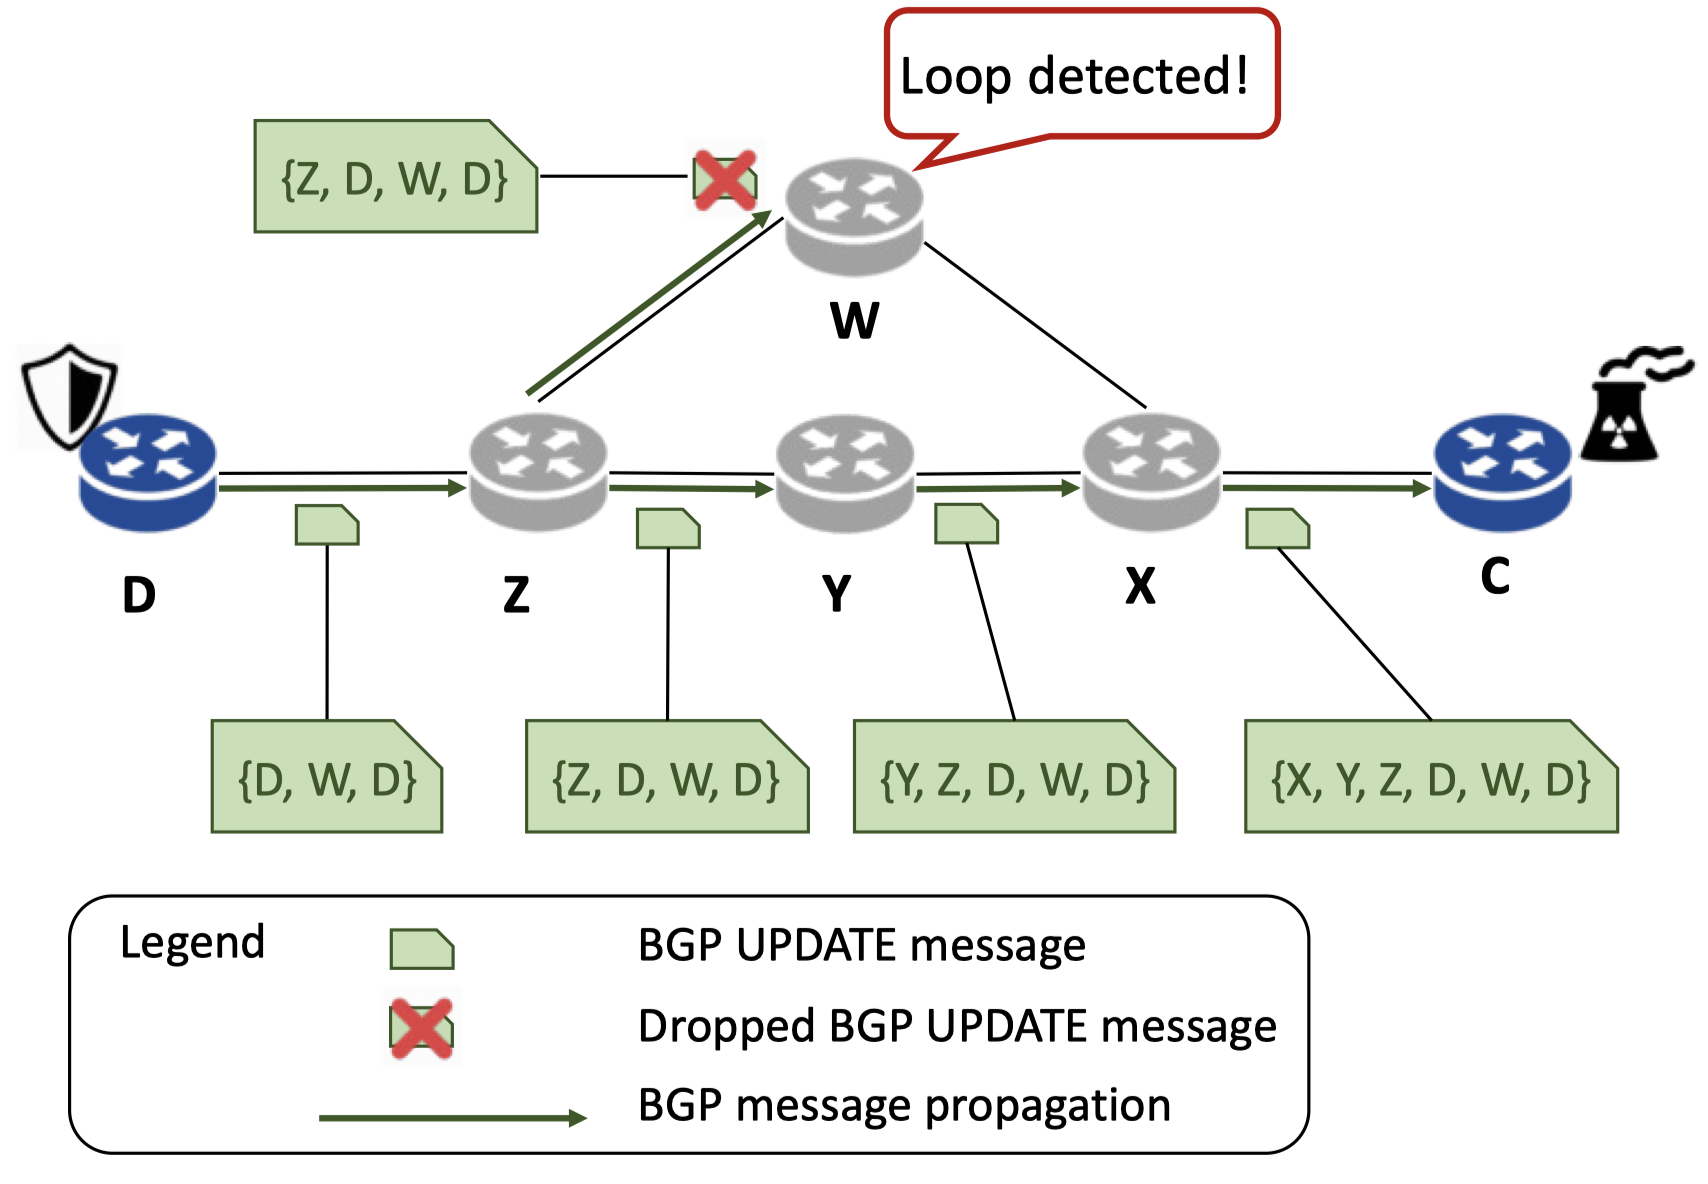
\includegraphics[scale=0.25]{figures/Defense.png}
  \caption{RAC防御示意图}
  \label{fig:Denfense}
\end{figure}

虽然上述的RAC防御模式在理论上是可行的,但是本论文从实际Internet应用的角度论证了在现实
中该技术方案的不可行性,不可行的原因文章从以下几个方面进行了论述:

\begin{itemize}
  \item 在实际应用之中,如果要做到对关键源结点的路由路径隔离,RAC需要毒化规避的自治系统
  数目实际在数千个;理论的BGP协议中可以附带约2000个结点的毒化,但是实际上限于路由器厂商
  技术建议、路由器系统实现以及ISP服务商的安全限制,实际的BGP路由更新仅允许附带255个结
  点的毒化;
  \item 如果弱化对关键源结点路由路径的绝对隔离要求,允许存在一定的路径泄漏,基于作者实现
  的一组贪心策略,通过实验可以发现在仅允许255个毒化约束下,RAC并不能够为关键数据流提供
  一个很好的洪泛攻击防御。
\end{itemize}

后续作者还设计了一个针对RAC重路由洪泛攻击防御策略的攻击模型,通过模拟实验验证了路径泄漏的
易发觉性、路由毒化后导致后续网络收敛困难、实际255个结点毒化约束下可行候选路由旁路过少等问题。

总的来说,本文的一个最大的突出点在于作者对于实际技术进行分析时,没有局限于基本的理论情形,
而是将技术放到了实际的运用场景之中进行分析,具备了更强的现实价值。另外文章通过对现实中技术
问题的挖掘,可以分析得到理论协议到实际应用的瓶颈所在,在这里是ISP服务商的限制和路由器制造
厂商的简化实现。另一点是文章突出强调了新的安全技术、网络协议在设计之中需要一个真实的评估
场景,这样才能得到一个更加实际有效的技术方案。

纵观全文,个人觉得文章还是存在着一定可以改进的地方。在论证关于弱化对关键源结点路由路径的绝对
隔离要求部分时,作者使用了自己设计的一套贪心策略来执行毒化结点的选择,并基于上述算法进行了
后续的一系列实验评估,试图说明即便弱化绝对路径隔离这一要求也很难为关键数据流形成一个良好的
洪泛攻击防御。虽然这样的贪心近似算法直观上是合理的,且文章阐述了该问题
的最优解是一个NP完全问题,但是这让读者很难相信是否存在另一个同样合理的策略使得得到的解是一个
能够有效抵御洪泛的情况。个人觉得如果可以加上更加严谨的数学论证,找到NP问题近似算法的一个最坏
近似比,这样使得后续的说明论证能够更加有力。

\vspace{200pt}

\end{document}